\documentclass[11pt]{article}

    %\usepackage[breakable]{tcolorbox}
    \usepackage[most]{tcolorbox}
    \usepackage{lmodern} 
    \usepackage{parskip} % Stop auto-indenting (to mimic markdown behaviour)
    
    \usepackage{iftex}
    \ifPDFTeX
    	\usepackage[T1]{fontenc}
    	\usepackage{mathpazo}
    \else
    	\usepackage{fontspec}
    \fi

    % Basic figure setup, for now with no caption control since it's done
    % automatically by Pandoc (which extracts ![](path) syntax from Markdown).
    \usepackage{graphicx}
    % Maintain compatibility with old templates. Remove in nbconvert 6.0
    \let\Oldincludegraphics\includegraphics
    % Ensure that by default, figures have no caption (until we provide a
    % proper Figure object with a Caption API and a way to capture that
    % in the conversion process - todo).
    \usepackage{caption}
    \DeclareCaptionFormat{nocaption}{}
    \captionsetup{format=nocaption,aboveskip=0pt,belowskip=0pt}

    \usepackage{float}
    \floatplacement{figure}{H} % forces figures to be placed at the correct location
    \usepackage{xcolor} % Allow colors to be defined
    \usepackage{enumerate} % Needed for markdown enumerations to work
    \usepackage{geometry} % Used to adjust the document margins
    \usepackage{amsmath} % Equations
    \usepackage{amssymb} % Equations
    \usepackage{textcomp} % defines textquotesingle
    % Hack from http://tex.stackexchange.com/a/47451/13684:
    \AtBeginDocument{%
        \def\PYZsq{\textquotesingle}% Upright quotes in Pygmentized code
    }
    \usepackage{upquote} % Upright quotes for verbatim code
    \usepackage{eurosym} % defines \euro
    \usepackage[mathletters]{ucs} % Extended unicode (utf-8) support
    \usepackage{fancyvrb} % verbatim replacement that allows latex
    \usepackage{grffile} % extends the file name processing of package graphics 
                         % to support a larger range
    \makeatletter % fix for old versions of grffile with XeLaTeX
    \@ifpackagelater{grffile}{2019/11/01}
    {
      % Do nothing on new versions
    }
    {
      \def\Gread@@xetex#1{%
        \IfFileExists{"\Gin@base".bb}%
        {\Gread@eps{\Gin@base.bb}}%
        {\Gread@@xetex@aux#1}%
      }
    }
    \makeatother
    \usepackage[Export]{adjustbox} % Used to constrain images to a maximum size
    \adjustboxset{max size={0.9\linewidth}{0.9\paperheight}}

    % The hyperref package gives us a pdf with properly built
    % internal navigation ('pdf bookmarks' for the table of contents,
    % internal cross-reference links, web links for URLs, etc.)
    \usepackage{hyperref}
    % The default LaTeX title has an obnoxious amount of whitespace. By default,
    % titling removes some of it. It also provides customization options.
    \usepackage{titling}
    \usepackage{longtable} % longtable support required by pandoc >1.10
    \usepackage{booktabs}  % table support for pandoc > 1.12.2
    \usepackage[inline]{enumitem} % IRkernel/repr support (it uses the enumerate* environment)
    \usepackage[normalem]{ulem} % ulem is needed to support strikethroughs (\sout)
                                % normalem makes italics be italics, not underlines
    \usepackage{mathrsfs}
    
\usepackage{fancyhdr}
\usepackage{lastpage}
\usepackage{cclicenses}

    % Colors for the hyperref package
    \definecolor{urlcolor}{rgb}{0,.145,.698}
    \definecolor{linkcolor}{rgb}{.71,0.21,0.01}
    \definecolor{citecolor}{rgb}{.12,.54,.11}

    % ANSI colors
    \definecolor{ansi-black}{HTML}{3E424D}
    \definecolor{ansi-black-intense}{HTML}{282C36}
    \definecolor{ansi-red}{HTML}{E75C58}
    \definecolor{ansi-red-intense}{HTML}{B22B31}
    \definecolor{ansi-green}{HTML}{00A250}
    \definecolor{ansi-green-intense}{HTML}{007427}
    \definecolor{ansi-yellow}{HTML}{DDB62B}
    \definecolor{ansi-yellow-intense}{HTML}{B27D12}
    \definecolor{ansi-blue}{HTML}{208FFB}
    \definecolor{ansi-blue-intense}{HTML}{0065CA}
    \definecolor{ansi-magenta}{HTML}{D160C4}
    \definecolor{ansi-magenta-intense}{HTML}{A03196}
    \definecolor{ansi-cyan}{HTML}{60C6C8}
    \definecolor{ansi-cyan-intense}{HTML}{258F8F}
    \definecolor{ansi-white}{HTML}{C5C1B4}
    \definecolor{ansi-white-intense}{HTML}{A1A6B2}
    \definecolor{ansi-default-inverse-fg}{HTML}{FFFFFF}
    \definecolor{ansi-default-inverse-bg}{HTML}{000000}

    % common color for the border for error outputs.
    \definecolor{outerrorbackground}{HTML}{FFDFDF}

    % commands and environments needed by pandoc snippets
    % extracted from the output of `pandoc -s`
    \providecommand{\tightlist}{%
      \setlength{\itemsep}{0pt}\setlength{\parskip}{0pt}}
    \DefineVerbatimEnvironment{Highlighting}{Verbatim}{commandchars=\\\{\}}
    % Add ',fontsize=\small' for more characters per line
    \newenvironment{Shaded}{}{}
    \newcommand{\KeywordTok}[1]{\textcolor[rgb]{0.00,0.44,0.13}{\textbf{{#1}}}}
    \newcommand{\DataTypeTok}[1]{\textcolor[rgb]{0.56,0.13,0.00}{{#1}}}
    \newcommand{\DecValTok}[1]{\textcolor[rgb]{0.25,0.63,0.44}{{#1}}}
    \newcommand{\BaseNTok}[1]{\textcolor[rgb]{0.25,0.63,0.44}{{#1}}}
    \newcommand{\FloatTok}[1]{\textcolor[rgb]{0.25,0.63,0.44}{{#1}}}
    \newcommand{\CharTok}[1]{\textcolor[rgb]{0.25,0.44,0.63}{{#1}}}
    \newcommand{\StringTok}[1]{\textcolor[rgb]{0.25,0.44,0.63}{{#1}}}
    \newcommand{\CommentTok}[1]{\textcolor[rgb]{0.38,0.63,0.69}{\textit{{#1}}}}
    \newcommand{\OtherTok}[1]{\textcolor[rgb]{0.00,0.44,0.13}{{#1}}}
    \newcommand{\AlertTok}[1]{\textcolor[rgb]{1.00,0.00,0.00}{\textbf{{#1}}}}
    \newcommand{\FunctionTok}[1]{\textcolor[rgb]{0.02,0.16,0.49}{{#1}}}
    \newcommand{\RegionMarkerTok}[1]{{#1}}
    \newcommand{\ErrorTok}[1]{\textcolor[rgb]{1.00,0.00,0.00}{\textbf{{#1}}}}
    \newcommand{\NormalTok}[1]{{#1}}
    
    % Additional commands for more recent versions of Pandoc
    \newcommand{\ConstantTok}[1]{\textcolor[rgb]{0.53,0.00,0.00}{{#1}}}
    \newcommand{\SpecialCharTok}[1]{\textcolor[rgb]{0.25,0.44,0.63}{{#1}}}
    \newcommand{\VerbatimStringTok}[1]{\textcolor[rgb]{0.25,0.44,0.63}{{#1}}}
    \newcommand{\SpecialStringTok}[1]{\textcolor[rgb]{0.73,0.40,0.53}{{#1}}}
    \newcommand{\ImportTok}[1]{{#1}}
    \newcommand{\DocumentationTok}[1]{\textcolor[rgb]{0.73,0.13,0.13}{\textit{{#1}}}}
    \newcommand{\AnnotationTok}[1]{\textcolor[rgb]{0.38,0.63,0.69}{\textbf{\textit{{#1}}}}}
    \newcommand{\CommentVarTok}[1]{\textcolor[rgb]{0.38,0.63,0.69}{\textbf{\textit{{#1}}}}}
    \newcommand{\VariableTok}[1]{\textcolor[rgb]{0.10,0.09,0.49}{{#1}}}
    \newcommand{\ControlFlowTok}[1]{\textcolor[rgb]{0.00,0.44,0.13}{\textbf{{#1}}}}
    \newcommand{\OperatorTok}[1]{\textcolor[rgb]{0.40,0.40,0.40}{{#1}}}
    \newcommand{\BuiltInTok}[1]{{#1}}
    \newcommand{\ExtensionTok}[1]{{#1}}
    \newcommand{\PreprocessorTok}[1]{\textcolor[rgb]{0.74,0.48,0.00}{{#1}}}
    \newcommand{\AttributeTok}[1]{\textcolor[rgb]{0.49,0.56,0.16}{{#1}}}
    \newcommand{\InformationTok}[1]{\textcolor[rgb]{0.38,0.63,0.69}{\textbf{\textit{{#1}}}}}
    \newcommand{\WarningTok}[1]{\textcolor[rgb]{0.38,0.63,0.69}{\textbf{\textit{{#1}}}}}
    
    % Slightly bigger margins than the latex defaults
    
    \geometry{verbose,tmargin=0.7in,bmargin=0.7in,lmargin=0.7in,rmargin=0.7in}
        
    % Define a nice break command that doesn't care if a line doesn't already
    % exist.
    \def\br{\hspace*{\fill} \\* }
    % Math Jax compatibility definitions
    \def\gt{>}
    \def\lt{<}
    \let\Oldtex\TeX
    \let\Oldlatex\LaTeX
    \renewcommand{\TeX}{\textrm{\Oldtex}}
    \renewcommand{\LaTeX}{\textrm{\Oldlatex}}
    % Document parameters
    % Document title
    \title{Opérateurs logiques}
      \date{Octobre 2021}  
	%\author{Yannick Chistel}
    
\makeatletter         
\renewcommand\maketitle[1]{
\hrule\medskip
{\raggedright % Note the extra {
\begin{center}
{\Huge \bfseries \sffamily #1 }\\[4ex] 
%{\Large  \@author}\\[2ex] 
%\@date\\[4ex]
\hrule \bigskip
\end{center}}} % Note the extra }
\makeatother    



\pagestyle{fancy}
\fancyhead{}
\renewcommand\headrulewidth{0pt}
\renewcommand\footrulewidth{1pt}
\fancyfoot[L]{YC}
\fancyfoot[C]{\thepage}
\fancyfoot[R]{\cc-\ccby-\ccnc}

% 
%\newtcolorbox{exemple}[2][]{
%    enhanced,
%    size=fbox,sharp corners,
%    colback=white,colframe=black,
%    colbacktitle=black,fonttitle=\bfseries,
%    attach boxed title to top left={yshift=-3mm,yshifttext=-3mm},
%    boxed title style={size=small,left=0pt,right=0pt,sharp corners},title=#2,#1}

\newtcolorbox{remarque}[2][]{colback=red!4!white,
colframe=red!64!black,fonttitle=\bfseries,
colbacktitle=red!64!black,enhanced,
attach boxed title to top left={xshift=4mm,yshift=-2mm},
title=#2,#1}  


\newtcolorbox{exemple}[2][]{colback=blue!4!white,
colframe=blue!64!green,fonttitle=\bfseries,
colbacktitle=blue!64!green,enhanced,
attach boxed title to top left={xshift=4mm,yshift=-2mm},
title=#2,#1}  
    
% Pygments definitions
\makeatletter
\def\PY@reset{\let\PY@it=\relax \let\PY@bf=\relax%
    \let\PY@ul=\relax \let\PY@tc=\relax%
    \let\PY@bc=\relax \let\PY@ff=\relax}
\def\PY@tok#1{\csname PY@tok@#1\endcsname}
\def\PY@toks#1+{\ifx\relax#1\empty\else%
    \PY@tok{#1}\expandafter\PY@toks\fi}
\def\PY@do#1{\PY@bc{\PY@tc{\PY@ul{%
    \PY@it{\PY@bf{\PY@ff{#1}}}}}}}
\def\PY#1#2{\PY@reset\PY@toks#1+\relax+\PY@do{#2}}

\@namedef{PY@tok@w}{\def\PY@tc##1{\textcolor[rgb]{0.73,0.73,0.73}{##1}}}
\@namedef{PY@tok@c}{\let\PY@it=\textit\def\PY@tc##1{\textcolor[rgb]{0.25,0.50,0.50}{##1}}}
\@namedef{PY@tok@cp}{\def\PY@tc##1{\textcolor[rgb]{0.74,0.48,0.00}{##1}}}
\@namedef{PY@tok@k}{\let\PY@bf=\textbf\def\PY@tc##1{\textcolor[rgb]{0.00,0.50,0.00}{##1}}}
\@namedef{PY@tok@kp}{\def\PY@tc##1{\textcolor[rgb]{0.00,0.50,0.00}{##1}}}
\@namedef{PY@tok@kt}{\def\PY@tc##1{\textcolor[rgb]{0.69,0.00,0.25}{##1}}}
\@namedef{PY@tok@o}{\def\PY@tc##1{\textcolor[rgb]{0.40,0.40,0.40}{##1}}}
\@namedef{PY@tok@ow}{\let\PY@bf=\textbf\def\PY@tc##1{\textcolor[rgb]{0.67,0.13,1.00}{##1}}}
\@namedef{PY@tok@nb}{\def\PY@tc##1{\textcolor[rgb]{0.00,0.50,0.00}{##1}}}
\@namedef{PY@tok@nf}{\def\PY@tc##1{\textcolor[rgb]{0.00,0.00,1.00}{##1}}}
\@namedef{PY@tok@nc}{\let\PY@bf=\textbf\def\PY@tc##1{\textcolor[rgb]{0.00,0.00,1.00}{##1}}}
\@namedef{PY@tok@nn}{\let\PY@bf=\textbf\def\PY@tc##1{\textcolor[rgb]{0.00,0.00,1.00}{##1}}}
\@namedef{PY@tok@ne}{\let\PY@bf=\textbf\def\PY@tc##1{\textcolor[rgb]{0.82,0.25,0.23}{##1}}}
\@namedef{PY@tok@nv}{\def\PY@tc##1{\textcolor[rgb]{0.10,0.09,0.49}{##1}}}
\@namedef{PY@tok@no}{\def\PY@tc##1{\textcolor[rgb]{0.53,0.00,0.00}{##1}}}
\@namedef{PY@tok@nl}{\def\PY@tc##1{\textcolor[rgb]{0.63,0.63,0.00}{##1}}}
\@namedef{PY@tok@ni}{\let\PY@bf=\textbf\def\PY@tc##1{\textcolor[rgb]{0.60,0.60,0.60}{##1}}}
\@namedef{PY@tok@na}{\def\PY@tc##1{\textcolor[rgb]{0.49,0.56,0.16}{##1}}}
\@namedef{PY@tok@nt}{\let\PY@bf=\textbf\def\PY@tc##1{\textcolor[rgb]{0.00,0.50,0.00}{##1}}}
\@namedef{PY@tok@nd}{\def\PY@tc##1{\textcolor[rgb]{0.67,0.13,1.00}{##1}}}
\@namedef{PY@tok@s}{\def\PY@tc##1{\textcolor[rgb]{0.73,0.13,0.13}{##1}}}
\@namedef{PY@tok@sd}{\let\PY@it=\textit\def\PY@tc##1{\textcolor[rgb]{0.73,0.13,0.13}{##1}}}
\@namedef{PY@tok@si}{\let\PY@bf=\textbf\def\PY@tc##1{\textcolor[rgb]{0.73,0.40,0.53}{##1}}}
\@namedef{PY@tok@se}{\let\PY@bf=\textbf\def\PY@tc##1{\textcolor[rgb]{0.73,0.40,0.13}{##1}}}
\@namedef{PY@tok@sr}{\def\PY@tc##1{\textcolor[rgb]{0.73,0.40,0.53}{##1}}}
\@namedef{PY@tok@ss}{\def\PY@tc##1{\textcolor[rgb]{0.10,0.09,0.49}{##1}}}
\@namedef{PY@tok@sx}{\def\PY@tc##1{\textcolor[rgb]{0.00,0.50,0.00}{##1}}}
\@namedef{PY@tok@m}{\def\PY@tc##1{\textcolor[rgb]{0.40,0.40,0.40}{##1}}}
\@namedef{PY@tok@gh}{\let\PY@bf=\textbf\def\PY@tc##1{\textcolor[rgb]{0.00,0.00,0.50}{##1}}}
\@namedef{PY@tok@gu}{\let\PY@bf=\textbf\def\PY@tc##1{\textcolor[rgb]{0.50,0.00,0.50}{##1}}}
\@namedef{PY@tok@gd}{\def\PY@tc##1{\textcolor[rgb]{0.63,0.00,0.00}{##1}}}
\@namedef{PY@tok@gi}{\def\PY@tc##1{\textcolor[rgb]{0.00,0.63,0.00}{##1}}}
\@namedef{PY@tok@gr}{\def\PY@tc##1{\textcolor[rgb]{1.00,0.00,0.00}{##1}}}
\@namedef{PY@tok@ge}{\let\PY@it=\textit}
\@namedef{PY@tok@gs}{\let\PY@bf=\textbf}
\@namedef{PY@tok@gp}{\let\PY@bf=\textbf\def\PY@tc##1{\textcolor[rgb]{0.00,0.00,0.50}{##1}}}
\@namedef{PY@tok@go}{\def\PY@tc##1{\textcolor[rgb]{0.53,0.53,0.53}{##1}}}
\@namedef{PY@tok@gt}{\def\PY@tc##1{\textcolor[rgb]{0.00,0.27,0.87}{##1}}}
\@namedef{PY@tok@err}{\def\PY@bc##1{{\setlength{\fboxsep}{\string -\fboxrule}\fcolorbox[rgb]{1.00,0.00,0.00}{1,1,1}{\strut ##1}}}}
\@namedef{PY@tok@kc}{\let\PY@bf=\textbf\def\PY@tc##1{\textcolor[rgb]{0.00,0.50,0.00}{##1}}}
\@namedef{PY@tok@kd}{\let\PY@bf=\textbf\def\PY@tc##1{\textcolor[rgb]{0.00,0.50,0.00}{##1}}}
\@namedef{PY@tok@kn}{\let\PY@bf=\textbf\def\PY@tc##1{\textcolor[rgb]{0.00,0.50,0.00}{##1}}}
\@namedef{PY@tok@kr}{\let\PY@bf=\textbf\def\PY@tc##1{\textcolor[rgb]{0.00,0.50,0.00}{##1}}}
\@namedef{PY@tok@bp}{\def\PY@tc##1{\textcolor[rgb]{0.00,0.50,0.00}{##1}}}
\@namedef{PY@tok@fm}{\def\PY@tc##1{\textcolor[rgb]{0.00,0.00,1.00}{##1}}}
\@namedef{PY@tok@vc}{\def\PY@tc##1{\textcolor[rgb]{0.10,0.09,0.49}{##1}}}
\@namedef{PY@tok@vg}{\def\PY@tc##1{\textcolor[rgb]{0.10,0.09,0.49}{##1}}}
\@namedef{PY@tok@vi}{\def\PY@tc##1{\textcolor[rgb]{0.10,0.09,0.49}{##1}}}
\@namedef{PY@tok@vm}{\def\PY@tc##1{\textcolor[rgb]{0.10,0.09,0.49}{##1}}}
\@namedef{PY@tok@sa}{\def\PY@tc##1{\textcolor[rgb]{0.73,0.13,0.13}{##1}}}
\@namedef{PY@tok@sb}{\def\PY@tc##1{\textcolor[rgb]{0.73,0.13,0.13}{##1}}}
\@namedef{PY@tok@sc}{\def\PY@tc##1{\textcolor[rgb]{0.73,0.13,0.13}{##1}}}
\@namedef{PY@tok@dl}{\def\PY@tc##1{\textcolor[rgb]{0.73,0.13,0.13}{##1}}}
\@namedef{PY@tok@s2}{\def\PY@tc##1{\textcolor[rgb]{0.73,0.13,0.13}{##1}}}
\@namedef{PY@tok@sh}{\def\PY@tc##1{\textcolor[rgb]{0.73,0.13,0.13}{##1}}}
\@namedef{PY@tok@s1}{\def\PY@tc##1{\textcolor[rgb]{0.73,0.13,0.13}{##1}}}
\@namedef{PY@tok@mb}{\def\PY@tc##1{\textcolor[rgb]{0.40,0.40,0.40}{##1}}}
\@namedef{PY@tok@mf}{\def\PY@tc##1{\textcolor[rgb]{0.40,0.40,0.40}{##1}}}
\@namedef{PY@tok@mh}{\def\PY@tc##1{\textcolor[rgb]{0.40,0.40,0.40}{##1}}}
\@namedef{PY@tok@mi}{\def\PY@tc##1{\textcolor[rgb]{0.40,0.40,0.40}{##1}}}
\@namedef{PY@tok@il}{\def\PY@tc##1{\textcolor[rgb]{0.40,0.40,0.40}{##1}}}
\@namedef{PY@tok@mo}{\def\PY@tc##1{\textcolor[rgb]{0.40,0.40,0.40}{##1}}}
\@namedef{PY@tok@ch}{\let\PY@it=\textit\def\PY@tc##1{\textcolor[rgb]{0.25,0.50,0.50}{##1}}}
\@namedef{PY@tok@cm}{\let\PY@it=\textit\def\PY@tc##1{\textcolor[rgb]{0.25,0.50,0.50}{##1}}}
\@namedef{PY@tok@cpf}{\let\PY@it=\textit\def\PY@tc##1{\textcolor[rgb]{0.25,0.50,0.50}{##1}}}
\@namedef{PY@tok@c1}{\let\PY@it=\textit\def\PY@tc##1{\textcolor[rgb]{0.25,0.50,0.50}{##1}}}
\@namedef{PY@tok@cs}{\let\PY@it=\textit\def\PY@tc##1{\textcolor[rgb]{0.25,0.50,0.50}{##1}}}

\def\PYZbs{\char`\\}
\def\PYZus{\char`\_}
\def\PYZob{\char`\{}
\def\PYZcb{\char`\}}
\def\PYZca{\char`\^}
\def\PYZam{\char`\&}
\def\PYZlt{\char`\<}
\def\PYZgt{\char`\>}
\def\PYZsh{\char`\#}
\def\PYZpc{\char`\%}
\def\PYZdl{\char`\$}
\def\PYZhy{\char`\-}
\def\PYZsq{\char`\'}
\def\PYZdq{\char`\"}
\def\PYZti{\char`\~}
% for compatibility with earlier versions
\def\PYZat{@}
\def\PYZlb{[}
\def\PYZrb{]}
\makeatother


    % For linebreaks inside Verbatim environment from package fancyvrb. 
    \makeatletter
        \newbox\Wrappedcontinuationbox 
        \newbox\Wrappedvisiblespacebox 
        \newcommand*\Wrappedvisiblespace {\textcolor{red}{\textvisiblespace}} 
        \newcommand*\Wrappedcontinuationsymbol {\textcolor{red}{\llap{\tiny$\m@th\hookrightarrow$}}} 
        \newcommand*\Wrappedcontinuationindent {3ex } 
        \newcommand*\Wrappedafterbreak {\kern\Wrappedcontinuationindent\copy\Wrappedcontinuationbox} 
        % Take advantage of the already applied Pygments mark-up to insert 
        % potential linebreaks for TeX processing. 
        %        {, <, #, %, $, ' and ": go to next line. 
        %        _, }, ^, &, >, - and ~: stay at end of broken line. 
        % Use of \textquotesingle for straight quote. 
        \newcommand*\Wrappedbreaksatspecials {% 
            \def\PYGZus{\discretionary{\char`\_}{\Wrappedafterbreak}{\char`\_}}% 
            \def\PYGZob{\discretionary{}{\Wrappedafterbreak\char`\{}{\char`\{}}% 
            \def\PYGZcb{\discretionary{\char`\}}{\Wrappedafterbreak}{\char`\}}}% 
            \def\PYGZca{\discretionary{\char`\^}{\Wrappedafterbreak}{\char`\^}}% 
            \def\PYGZam{\discretionary{\char`\&}{\Wrappedafterbreak}{\char`\&}}% 
            \def\PYGZlt{\discretionary{}{\Wrappedafterbreak\char`\<}{\char`\<}}% 
            \def\PYGZgt{\discretionary{\char`\>}{\Wrappedafterbreak}{\char`\>}}% 
            \def\PYGZsh{\discretionary{}{\Wrappedafterbreak\char`\#}{\char`\#}}% 
            \def\PYGZpc{\discretionary{}{\Wrappedafterbreak\char`\%}{\char`\%}}% 
            \def\PYGZdl{\discretionary{}{\Wrappedafterbreak\char`\$}{\char`\$}}% 
            \def\PYGZhy{\discretionary{\char`\-}{\Wrappedafterbreak}{\char`\-}}% 
            \def\PYGZsq{\discretionary{}{\Wrappedafterbreak\textquotesingle}{\textquotesingle}}% 
            \def\PYGZdq{\discretionary{}{\Wrappedafterbreak\char`\"}{\char`\"}}% 
            \def\PYGZti{\discretionary{\char`\~}{\Wrappedafterbreak}{\char`\~}}% 
        } 
        % Some characters . , ; ? ! / are not pygmentized. 
        % This macro makes them "active" and they will insert potential linebreaks 
        \newcommand*\Wrappedbreaksatpunct {% 
            \lccode`\~`\.\lowercase{\def~}{\discretionary{\hbox{\char`\.}}{\Wrappedafterbreak}{\hbox{\char`\.}}}% 
            \lccode`\~`\,\lowercase{\def~}{\discretionary{\hbox{\char`\,}}{\Wrappedafterbreak}{\hbox{\char`\,}}}% 
            \lccode`\~`\;\lowercase{\def~}{\discretionary{\hbox{\char`\;}}{\Wrappedafterbreak}{\hbox{\char`\;}}}% 
            \lccode`\~`\:\lowercase{\def~}{\discretionary{\hbox{\char`\:}}{\Wrappedafterbreak}{\hbox{\char`\:}}}% 
            \lccode`\~`\?\lowercase{\def~}{\discretionary{\hbox{\char`\?}}{\Wrappedafterbreak}{\hbox{\char`\?}}}% 
            \lccode`\~`\!\lowercase{\def~}{\discretionary{\hbox{\char`\!}}{\Wrappedafterbreak}{\hbox{\char`\!}}}% 
            \lccode`\~`\/\lowercase{\def~}{\discretionary{\hbox{\char`\/}}{\Wrappedafterbreak}{\hbox{\char`\/}}}% 
            \catcode`\.\active
            \catcode`\,\active 
            \catcode`\;\active
            \catcode`\:\active
            \catcode`\?\active
            \catcode`\!\active
            \catcode`\/\active 
            \lccode`\~`\~ 	
        }
    \makeatother

    \let\OriginalVerbatim=\Verbatim
    \makeatletter
    \renewcommand{\Verbatim}[1][1]{%
        %\parskip\z@skip
        \sbox\Wrappedcontinuationbox {\Wrappedcontinuationsymbol}%
        \sbox\Wrappedvisiblespacebox {\FV@SetupFont\Wrappedvisiblespace}%
        \def\FancyVerbFormatLine ##1{\hsize\linewidth
            \vtop{\raggedright\hyphenpenalty\z@\exhyphenpenalty\z@
                \doublehyphendemerits\z@\finalhyphendemerits\z@
                \strut ##1\strut}%
        }%
        % If the linebreak is at a space, the latter will be displayed as visible
        % space at end of first line, and a continuation symbol starts next line.
        % Stretch/shrink are however usually zero for typewriter font.
        \def\FV@Space {%
            \nobreak\hskip\z@ plus\fontdimen3\font minus\fontdimen4\font
            \discretionary{\copy\Wrappedvisiblespacebox}{\Wrappedafterbreak}
            {\kern\fontdimen2\font}%
        }%
        
        % Allow breaks at special characters using \PYG... macros.
        \Wrappedbreaksatspecials
        % Breaks at punctuation characters . , ; ? ! and / need catcode=\active 	
        \OriginalVerbatim[#1,codes*=\Wrappedbreaksatpunct]%
    }
    \makeatother

    % Exact colors from NB
    \definecolor{incolor}{HTML}{303F9F}
    \definecolor{outcolor}{HTML}{D84315}
    \definecolor{cellborder}{HTML}{CFCFCF}
    \definecolor{cellbackground}{HTML}{F7F7F7}
    
    % prompt
    \makeatletter
    \newcommand{\boxspacing}{\kern\kvtcb@left@rule\kern\kvtcb@boxsep}
    \makeatother
    \newcommand{\prompt}[4]{
        {\ttfamily\llap{{\color{#2}[#3]:\hspace{3pt}#4}}\vspace{-\baselineskip}}
    }
    

    
    % Prevent overflowing lines due to hard-to-break entities
    \sloppy 
    % Setup hyperref package
    \hypersetup{
      breaklinks=true,  % so long urls are correctly broken across lines
      colorlinks=true,
      urlcolor=urlcolor,
      linkcolor=linkcolor,
      citecolor=citecolor,
      }

    

\begin{document}
    
    \maketitle{Encodage des caractères}
    
    

%    
%    \hypertarget{encodage-des-caractuxe8res}{%
%\section{Encodage des caractères}\label{encodage-des-caractuxe8res}}

    \hypertarget{repruxe9sentation-des-textes}{%
\section{Représentation des textes}\label{repruxe9sentation-des-textes}}

La représentation des textes dans un ordinateur s'appuie sur un
encodage. Une table associe un nombre à chaque caractère. Les systèmes
d'exploitation possèdent ces tables et font la conversion en binaire.

L'informatique créée aux Etats-Unis, a pu se contenter 128 caractères en
anglais pendant longtemps, mais ces caractères sont devenus insuffisants
notamment avec les langues latines et leurs nombreux caratères
accentués. Les tables se sont alors agrandies et se sont harmonisées.
Mais d'autres langues, comme l'arabe, le corréen et le japonais qui
utilisent des caractères très particuliers, propres à leurs langues, ont
conduit à étendre encore les tables de caractères.

On peut retenir 3 tables de codage importantes :

\begin{itemize}
\tightlist
\item
  Le codage ASCII créé dans les années 1960.
\item
  La norme ISO 8859-1 et 8859-15
\item
  Le codage unicode et sa représentation en UTF-8
\end{itemize}

\hypertarget{le-codage-ascii}{%
\section{Le codage ASCII}\label{le-codage-ascii}}

La table de caratères ASCII (American Standard Code for Information
Interchange) a été élaborée au début des années 1960.

Cette norme définit un jeu de 128 caractères représenté par un octet,
mais seuls 7 bits sont utilisés d'où le nombre de caractères utilisés
puisque sur 7 bits on dispose de \(2^{7}=128\) valeurs différentes.

A chaque codage binaire d'un caractère est associé un nombre décimal
égal à cette valeur binaire convertie.

\hypertarget{exemple}{%
\subsubsection*{Exemple}\label{exemple}}

Voici quelques caractères de la table ASCII:

\begin{itemize}
\tightlist
\item
  Le caratère A, en majuscule, correspond au nombre décimal \(65_{10}\)
  dans la table ASCII que l'on note \(41_{16}\) en hexadécimal et de
  codage binaire \(01000001_{2}\).
\item
  Le caractère a, en minuscule, correspond au nombre décimal \(97_{10}\)
  dans la table ASCII que l'on note \(61_{16}\) en hexadécimal et de
  codage binaire \(01100001_{2}\).
\end{itemize}

\hypertarget{remarque}{%
\subsubsection*{Remarque}\label{remarque}}

La table ASCII contient des caractères spéciaux entre \(00\) et \(32\)
comme les caractères blancs (espace, tabulation, etc), retours à la
ligne, suppressions et des caractères de contrôle. Ce sont des
caractères non imprimables

A ces 32 caractères spéciaux, il y en a un dernier de valeur décimale
\(127_{10}\) qui correspond à la touche del du clavier.

\hypertarget{table-de-caractuxe8res-ascii}{%
\subsubsection*{Table de caractères
ASCII}\label{table-de-caractuxe8res-ascii}}

\begin{figure}
\centering
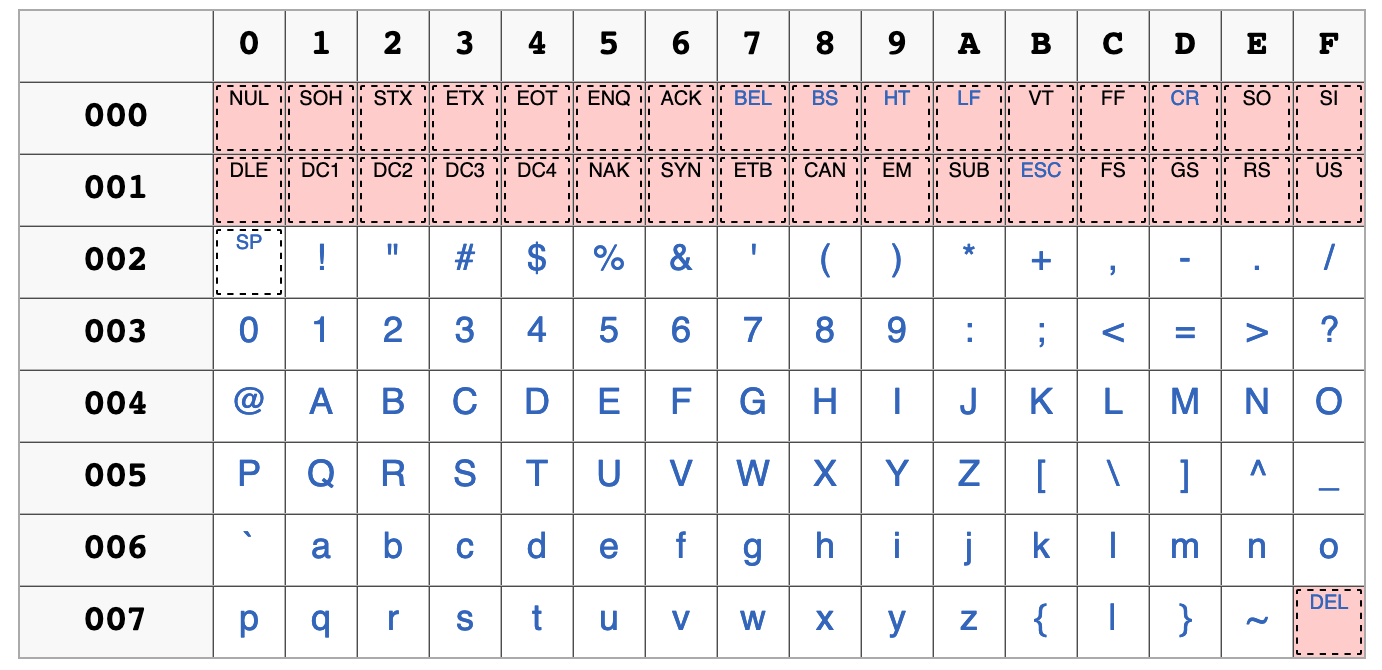
\includegraphics{img/tableASCII.png}
\caption{tableASCII.png}
\end{figure}

Cette table est à double entrée. La colonne de gauche représente les
trois premiers chiffres hexadécimaux et la première ligne le dernier
chiffre hexadécimal du codage du caractère.

On lit la table de la façon suivante:

\begin{itemize}
\tightlist
\item
  on repère le caractère dans la table situé à l'intersection d'une
  ligne et d'une colonne;
\item
  sur la ligne de ce caractère, on note les trois chiffres hexadécimaux
  de la première colonne;
\item
  sur la colonne de ce caratère, on note le chiffre hexadécimal de la
  première ligne.
\item
  on concatène les trois chiffres de la première colonne avec le chiffre
  de la première ligne.
\end{itemize}

\hypertarget{exemple-1}{%
\subsubsection*{Exemple}\label{exemple-1}}

\begin{itemize}
\tightlist
\item
  Le A est situé sur la ligne contenant les chiffres \(004\) (première
  colonne) et sur la colonne contenant le chiffre \(1\) (première
  ligne). Donc le caractère A est représenté par la valeur hexadécimale
  0041.
\item
  Le symbole \% est situé sur la ligne repérée \(002\) et sur la colonne
  repérée \(5\) donc il est représenté par le code hexadécimal \(0025\)
  et codé \(00100101\) en binaire.
\end{itemize}

\hypertarget{norme-iso-8859}{%
\section{Norme ISO 8859}\label{norme-iso-8859}}

Les caractères imprimables de la table ASCII sont devenus rapidement
insuffisants pour transmettre des textes dans d'autres langues que
l'anglais.

La table ASCII ne contient aucun caractère accentué ! Pour remédier à ce
problème l'ISO, \textbf{Organisme International de Normalisation} a
proposé la table ISO 8859 qui utilise 256 caractères sur un octet
complet

Pour définir le plus de caractères possible, la norme ISO définit
plusieurs tables 8859-n où n est le numéro de la table. Il y a 16 tables
pour les différentes langues.

En France, on a utilisé la table 8859-1, appelée aussi \emph{latin-1} et
considérée comme multi-langue et la table ISO-8859-15 qui introduit le
symbole monétaire € et qui gère mieux le français.

\hypertarget{remarque-1}{%
\subsubsection*{Remarque}\label{remarque-1}}

Toutes les tables ISO 8859-n contiennent les 128 caractères ASCII et 128
autres caractères propre à une langue (latine, arabe, grec, cyrillique,
hebreu, \ldots).

Il existe 10 tables différentes pour les langues latines !

\hypertarget{tables-de-caractuxe8res-iso-8859-1-et-8859-15}{%
\subsubsection*{Tables de caractères ISO 8859-1 et
8859-15}\label{tables-de-caractuxe8res-iso-8859-1-et-8859-15}}

\begin{figure}
\centering
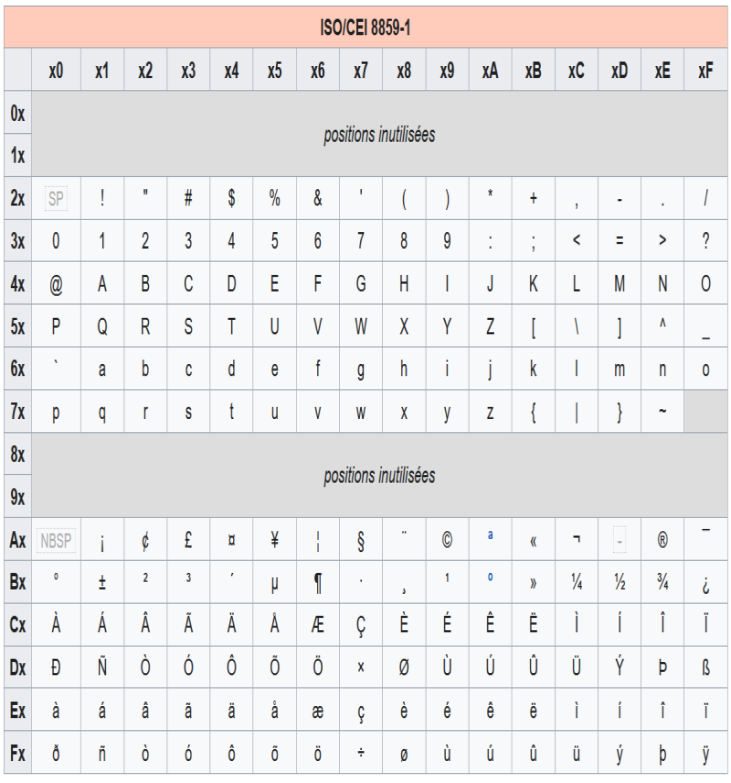
\includegraphics{img/iso-8859-1.png}
\caption{iso-8859-1.png}
\end{figure}

    \begin{figure}
\centering
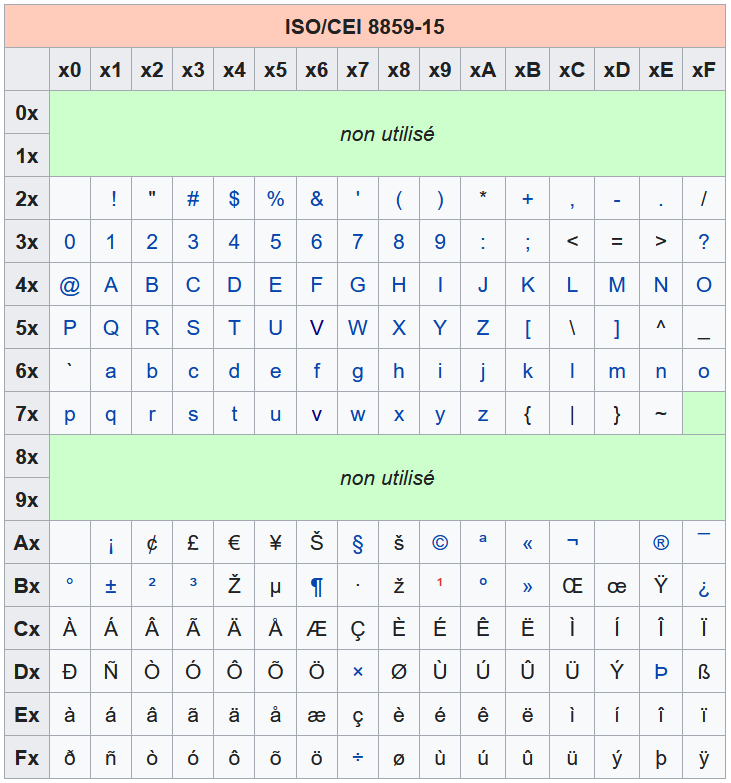
\includegraphics{img/iso-8859-15.png}
\caption{iso-8859-1.png}
\end{figure}

Les tables précédentes montrent que les 128 premiers caractères sont
ceux de la table ASCII. Finalement, on a complété la table ASCII avec
128 nouveaux caratères (selon les langues et pays).

On peut remarquer quelques différences entre les tables ISO 8859-1 et
ISO 8859-15 comme les fractions 1/4 et 1/2 peut utilisés en France et
remplacés par les caractère OE, oe collés.

    \hypertarget{la-norme-unicode}{%
\section{La norme Unicode}\label{la-norme-unicode}}

La norme ISO 8859 permet d'encoder un grand nombre de caractères mais
cela ne suffisait toujours pas. La multiplicité des tables rend
difficile la rédaction d'un texte en plusieurs langues qui utilisent
différentes tables ! Par exemple écrire un texte mélangeant le japonais
et le français.

L'ISO a donc défini un jeu universel de caractères sous la norme ISO
10646 appelée \textbf{UNICODE}.

Cette norme associe à chaque caractère (lettre, idéogramme,
emoji,\ldots) un \textbf{point de code}. Ce point de code est un
\textbf{numéro} en \textbf{hexadécimal} préfixé par \textbf{U+}.

\hypertarget{exemple}{%
\subsubsection*{Exemple}\label{exemple}}

\begin{itemize}
\tightlist
\item
  Le caractère ``A'' a pour point de code \textbf{U+0041} et nom unique
  \textbf{LATIN CAPITAL LETTER A} (on remarque que c'est sa valeur
  hexadécimale dans la table ASCII).
\item
  Le caractère ``?'' a pour point de code \textbf{U+003F} et nom unique
  \textbf{QUESTION MARK} (on remarque aussi que c'est sa valeur
  hexadécimale dans la table ASCII).
\end{itemize}

\textbf{Unicode} est une norme qui définit les techniques pour encoder
en binaire les \textbf{points de code} de façon plus ou moins
économique. Ces encodages sont appelés \textbf{Universal Transform
Format} et notés \textbf{UTF-n} où n désigne le nombre minimal de bits
pour représenter un point de code (n=8, 16 ou 32).

\textbf{UTF-8} est le format d'encodage qui utilise au minimum 8 bits
pour coder les caractères. Il est compatible avec la table de caractère
ASCII. Les 128 premiers points de code sont ceux de la table ASCII.

Selon les caractères et la valeur des points de code, l'encodage en
UTF-8 utilise 1, 2, 3 ou 4 octets.

Le tableau ci-dessous donne l'encodage des caratères en UTF-8.

\begin{longtable}[]{@{}ccc@{}}
\toprule
\textbf{Plage} & \textbf{Suite d'octets (en binaire)} & \textbf{Nombre
de bits utilisés}\tabularnewline
\midrule
\endhead
U+0000 à U+007F & 0xxxxxxx & 7 bits\tabularnewline
U+0080 à U+07FF & 110xxxxx 10xxxxxx & 11 bits\tabularnewline
U+0800 à U+FFFF & 1110xxxx 10xxxxxx 10xxxxxx & 16 bits\tabularnewline
U+10000 à U+10FFFF & 11110xxx 10xxxxx 10xxxxxx 10xxxxxx & 21
bits\tabularnewline
\bottomrule
\end{longtable}

\hypertarget{exemple-dencodage-en-utf-8}{%
\subsubsection*{Exemple d'encodage en
UTF-8}\label{exemple-dencodage-en-utf-8}}

\begin{enumerate}
\def\labelenumi{\arabic{enumi}.}
\item
  Commençons par un caractère ASCII dont le point de code est
  \textbf{U+005A}. On remarque que ce point de code appartient bien à la
  plage \([U+0000 ; U+007F]\) donc est codé sur 1 octet commençant par
  \(0\).\\
  En fait, il est encodé en UTF-8 comme en ASCII par la valeur binaire
  \(5A_{16} = 0101 1010_{2}\)
\item
  Prenons comme second exemple, un caractère accentué que l'on retrouve
  dans la table ISO 8859-15 dont le point de code est \textbf{U+00C9}.
  Le point de code appartient à la plage \([U+0080; U+07FF]\) donc il
  est encodé en UTF-8 sur 2 octets (contrairement à l'encodage ISO qui
  n'en utilisait qu'un seul). Comment est-il encodé en binaire ?
\end{enumerate}

\begin{quote}
L'encodage binaire sera de la forme \(110xxxxx~~10xxxxxx\) ou chaque x
représente un bit issu du point de code.

On convertit en binaire \(00C9_{16} = 0000~0000~~1100~1001_{2}\) et on
remplace chaque bit x par un bit de C9.

\begin{longtable}[]{@{}cccccccccccccccccc@{}}
\toprule
Sur 2 octets & 1 & 1 & 0 & x & x & x & x & x & & 1 & 0 & x & x & x & x &
x & x\tabularnewline
\midrule
\endhead
U+00C9 & & & & 0 & 0 & 0 & 1 & 1 & & & & 0 & 0 & 1 & 0 & 0 &
1\tabularnewline
UTF-8 & 1 & 1 & 0 & 0 & 0 & 0 & 1 & 1 & & 1 & 0 & 0 & 0 & 1 & 0 & 0 &
1\tabularnewline
\bottomrule
\end{longtable}

En écriture hexadécimale, le caractère de point de code \textbf{U+00C9}
est encodé en UTF-8 par \textbf{C3 89}.
\end{quote}

\begin{enumerate}
\def\labelenumi{\arabic{enumi}.}
\setcounter{enumi}{2}
\tightlist
\item
  Pour finir, le caractère de point de code \textbf{U+FFFD} appartient à
  la plage \([U+0800 ; U+FFFF]\). Ce caractère est donc encode en UTF-8
  sur trois octets. Comment est-il encodé en binaire ?
\end{enumerate}

\begin{quote}
L'encodage binaire sera de la forme \(1110xxxx~~10xxxxxx~~10xxxxxx\) ou
chaque x représente un bit issu du point de code.

On convertit en binaire \(FFFD_{16} = 1111~1111~~1111~1101_{2}\) et on
remplace chaque bit x par un bit de C9.

\begin{longtable}[]{@{}ccccccccccccccccccccccccccc@{}}
\toprule
Sur 3 octets & 1 & 1 & 1 & 0 & x & x & x & x & & 1 & 0 & x & x & x & x &
x & x & & 1 & 0 & x & x & x & x & x & x\tabularnewline
\midrule
\endhead
U+FFFD & & & & & 1 & 1 & 1 & 1 & & & & 1 & 1 & 1 & 1 & 1 & 1 & & & & 1 &
1 & 1 & 1 & 0 & 1\tabularnewline
UTF-8 & 1 & 1 & 1 & 0 & 1 & 1 & 1 & 1 & & 1 & 0 & 1 & 1 & 1 & 1 & 1 & 1
& & 1 & 0 & 1 & 1 & 1 & 1 & 0 & 1\tabularnewline
\bottomrule
\end{longtable}

En écriture hexadécimale, le caractère de point de code \textbf{U+FFFD}
est encodé en UTF-8 par \textbf{EF BF BD} soit �.
\end{quote}

    \hypertarget{remarque}{%
\subsubsection*{Remarque}\label{remarque}}

En python, on peut déclarer, sous réserve de coder en UTF-8, directement
un caractère par son point de code unicode.

Par exemple pour le symbole � : c=`\(\backslash uFFFD\)'

Il existe une méthode \textbf{encode()} qui donne le codage binaire noté
en hexadécimal d'un caratère dont on connait le point de code:

Avec c=`\(\backslash uFFFD\)' et en exécutant c.encode(), cela renvoie
\(b'\backslash xe2\backslash x82\backslash xac'\) qui est le code
hexadécimal de l'encodage en UTF-8 du caractère.

    \hypertarget{sitographie}{%
\subsection*{Sitographie}\label{sitographie}}

\begin{itemize}
\tightlist
\item
  Sur wikipedia :
  \href{https://fr.wikipedia.org/wiki/ISO/CEI_8859}{Norme ISO 8859}
\item
  Sur wikipedia : \href{https://fr.wikipedia.org/wiki/UTF-8}{UTF-8}
\end{itemize}

    \begin{tcolorbox}[breakable, size=fbox, boxrule=1pt, pad at break*=1mm,colback=cellbackground, colframe=cellborder]
\prompt{In}{incolor}{1}{\boxspacing}
\begin{Verbatim}[commandchars=\\\{\}]
\PY{n}{c}\PY{o}{=}\PY{l+s+s1}{\PYZsq{}}\PY{l+s+se}{\PYZbs{}u00c3}\PY{l+s+s1}{\PYZsq{}}
\PY{n}{c}\PY{o}{.}\PY{n}{encode}\PY{p}{(}\PY{p}{)}
\end{Verbatim}
\end{tcolorbox}

            \begin{tcolorbox}[breakable, size=fbox, boxrule=.5pt, pad at break*=1mm, opacityfill=0]
\prompt{Out}{outcolor}{1}{\boxspacing}
\begin{Verbatim}[commandchars=\\\{\}]
b'\textbackslash{}xc3\textbackslash{}x83'
\end{Verbatim}
\end{tcolorbox}
        
    \begin{tcolorbox}[breakable, size=fbox, boxrule=1pt, pad at break*=1mm,colback=cellbackground, colframe=cellborder]
\prompt{In}{incolor}{2}{\boxspacing}
\begin{Verbatim}[commandchars=\\\{\}]
\PY{n}{c}
\end{Verbatim}
\end{tcolorbox}

            \begin{tcolorbox}[breakable, size=fbox, boxrule=.5pt, pad at break*=1mm, opacityfill=0]
\prompt{Out}{outcolor}{2}{\boxspacing}
\begin{Verbatim}[commandchars=\\\{\}]
'Ã'
\end{Verbatim}
\end{tcolorbox}
        
    \begin{tcolorbox}[breakable, size=fbox, boxrule=1pt, pad at break*=1mm,colback=cellbackground, colframe=cellborder]
\prompt{In}{incolor}{3}{\boxspacing}
\begin{Verbatim}[commandchars=\\\{\}]
\PY{n}{p}\PY{o}{=}\PY{l+s+sa}{b}\PY{l+s+s1}{\PYZsq{}}\PY{l+s+se}{\PYZbs{}xc3}\PY{l+s+se}{\PYZbs{}xb8}\PY{l+s+s1}{\PYZsq{}}
\end{Verbatim}
\end{tcolorbox}

    \begin{tcolorbox}[breakable, size=fbox, boxrule=1pt, pad at break*=1mm,colback=cellbackground, colframe=cellborder]
\prompt{In}{incolor}{4}{\boxspacing}
\begin{Verbatim}[commandchars=\\\{\}]
\PY{n}{p}\PY{o}{.}\PY{n}{decode}\PY{p}{(}\PY{p}{)}
\end{Verbatim}
\end{tcolorbox}

            \begin{tcolorbox}[breakable, size=fbox, boxrule=.5pt, pad at break*=1mm, opacityfill=0]
\prompt{Out}{outcolor}{4}{\boxspacing}
\begin{Verbatim}[commandchars=\\\{\}]
'ø'
\end{Verbatim}
\end{tcolorbox}
        
    \begin{tcolorbox}[breakable, size=fbox, boxrule=1pt, pad at break*=1mm,colback=cellbackground, colframe=cellborder]
\prompt{In}{incolor}{5}{\boxspacing}
\begin{Verbatim}[commandchars=\\\{\}]
\PY{n}{c}\PY{o}{=}\PY{l+s+s1}{\PYZsq{}}\PY{l+s+se}{\PYZbs{}uFFFD}\PY{l+s+s1}{\PYZsq{}}
\PY{n}{c}\PY{o}{.}\PY{n}{encode}\PY{p}{(}\PY{p}{)}
\end{Verbatim}
\end{tcolorbox}

            \begin{tcolorbox}[breakable, size=fbox, boxrule=.5pt, pad at break*=1mm, opacityfill=0]
\prompt{Out}{outcolor}{5}{\boxspacing}
\begin{Verbatim}[commandchars=\\\{\}]
b'\textbackslash{}xef\textbackslash{}xbf\textbackslash{}xbd'
\end{Verbatim}
\end{tcolorbox}
        
    \begin{tcolorbox}[breakable, size=fbox, boxrule=1pt, pad at break*=1mm,colback=cellbackground, colframe=cellborder]
\prompt{In}{incolor}{6}{\boxspacing}
\begin{Verbatim}[commandchars=\\\{\}]
\PY{n}{c}
\end{Verbatim}
\end{tcolorbox}

            \begin{tcolorbox}[breakable, size=fbox, boxrule=.5pt, pad at break*=1mm, opacityfill=0]
\prompt{Out}{outcolor}{6}{\boxspacing}
\begin{Verbatim}[commandchars=\\\{\}]
'�'
\end{Verbatim}
\end{tcolorbox}
        
    \begin{tcolorbox}[breakable, size=fbox, boxrule=1pt, pad at break*=1mm,colback=cellbackground, colframe=cellborder]
\prompt{In}{incolor}{7}{\boxspacing}
\begin{Verbatim}[commandchars=\\\{\}]
\PY{n}{c}\PY{o}{=}\PY{l+s+s1}{\PYZsq{}}\PY{l+s+se}{\PYZbs{}u00e9}\PY{l+s+s1}{\PYZsq{}}
\end{Verbatim}
\end{tcolorbox}

    \begin{tcolorbox}[breakable, size=fbox, boxrule=1pt, pad at break*=1mm,colback=cellbackground, colframe=cellborder]
\prompt{In}{incolor}{8}{\boxspacing}
\begin{Verbatim}[commandchars=\\\{\}]
\PY{n}{c}\PY{o}{.}\PY{n}{encode}\PY{p}{(}\PY{p}{)}
\end{Verbatim}
\end{tcolorbox}

            \begin{tcolorbox}[breakable, size=fbox, boxrule=.5pt, pad at break*=1mm, opacityfill=0]
\prompt{Out}{outcolor}{8}{\boxspacing}
\begin{Verbatim}[commandchars=\\\{\}]
b'\textbackslash{}xc3\textbackslash{}xa9'
\end{Verbatim}
\end{tcolorbox}

    
    
    
\end{document}
